\section{Vildtskadebekendtgørelsen}

\begin{frame}
  \vspace{3em}
  \begin{center}
    {\LARGE \textbf{Vildtskadebekendtgørelsen}}
    \vspace{2em}
    \\ Bekendtgørelse om vildtskader
\par
{\normalsize \href{https://www.retsinformation.dk/eli/lta/2026/708}{BEK nr 708 af 27/08/2026}}
\vspace{0.5em}
\par
{\small Senest opdateret: 4.\ september 2026}
\vspace{1em}
\par
  \end{center}
\end{frame}
\begin{frame}{Læringsmål ift. vildskadebekendtgørelsen}

\textbf{Vildtskader}

\vspace{0.2cm}

Jagttegnsaspiranter skal kende:

\begin{itemize}
    \item \textbf{Bekendtgørelse nr. 1408 af 3. oktober 2022 om vildtskader}
    \begin{itemize}
        \item (vildtskadebekendtgørelsen)
        \item Hele bekendtgørelsen
    \end{itemize}

    \item \textbf{Lov om jagt og vildtforvaltning}, senest bekendtgjort ved
    lovbekendtgørelse nr. 639 af 26. maj 2023
    \begin{itemize}
        \item (jagt- og vildtforvaltningsloven)
        \item §§ 37 og 38
    \end{itemize}
\end{itemize}

\vspace{0.2cm}

Loven og bekendtgørelsen omhandler reglerne for regulering af vildt.

\vspace{0.2cm}

I jagtprøven kan der stilles spørgsmål til konkrete arter, tidspunkter og
situationer, hvor man kan opnå tilladelse til regulering (ringdue, råge, grågås,
krage, husskade, ræv, mink, mårhund, vaskebjørn, husmår, ilder, vildsvin).

\end{frame}


\begin{frame}{Jagt og regulering}

\vspace{1em}

\small

\raggedright

\begin{itemize}

\itemsep0.6em % Justér afstand mellem bullets

\item \textbf{Regulering} er målrettet funktionel ned/ombringelse af specifik type vildt i et område, hvor \textbf{jagt} er rekreativ nedlæggelse af vildt med jagttider.

\item Formål: beskytte menneskers og dyrs sundhed, smitte, luffartssikkerhed, beskytte flora og fauna, skade på ejendom/landbrug mm.

\item Regulering er koblet til ejeren/brugeren af ejendom (kan ikke besluttes af andre).

\item Indehaver af reguleringstilladelse kan bemyndige person med jagttegn til at udføre reguleringen.

\end{itemize}

\end{frame}

\begin{frame}{Regulering uden foregående aftale (tilladelse)}

\vspace{1em}

\small

\raggedright

\begin{itemize}

\itemsep0.6em % Justér afstand mellem bullets

\item \textbf{Hjortevildt og hare} kan reguleres hele året i forsvarligt indhegnede områder med erhvervsmæssig drift til plateskole, gartneri og frugtplantager.

\item \textbf{Husmår og ilder} kan regulerers hele året i fjerkræsindhegninger, beboelse og pelsdyrfarme. Afstand til bebyggelse/hegn: (fælder indtil 10 m /skydevåben 25 m).

\item \textbf{Ræv} kan reguleres fra 1/6 - 29/2 ved indhegninger til fjerkræ og smågrise (bebyggelse/hegn: fælder indtil 10 m /skydevåben 25 m). Skade på øvrig fauna 1-29/2. Rævehvalpe må reguleres 1/7-31/8 udenfor rævegraven (men ikke i områder hvor der er gennemført naturforbedringer i henhold til biotopplaner). Kan skydes fra jagttårne og -stiger fra 1 time før til 1 time efter med glatløbet haglgevær og riflede våben. 

\item \textbf{Vildkanin} Kan reguleres hele året, såfremt den forvolder skade.

\end{itemize}

\end{frame}

\begin{frame}{Regulering uden foregående aftale (tilladelse) - \textit{fortsat}}

\vspace{1em}

\small

\raggedright

\begin{itemize}

\itemsep0.6em % Justér afstand mellem bullets

\item \textbf{Vildsvin} kan reguleres hele året. Kan reguleres hele døgnet. Må skydes på foderpladsen med kunstigt lys etc. 

\item \textbf{Særlige arter} Invasive arter fastsættes af EU. Omfatter bl.a nilgås, bisamrotte, sikavildt, amerikansk skarveand, muntjak, mårhund m.fl.     


\end{itemize}

\end{frame}

\begin{frame}{Regulering efter forudgående tilladelse}

\vspace{1em}

\small

\raggedright

\begin{itemize}
\itemsep0.6em


\item \textbf{Råge (§ 12)}: Tilladelse til regulering i flokke på marker (1. juli–30. sept.), i kolonier før æglægning (15. jan.–15. marts), unger uden for rede (1. maj–15. juni), unger på marker (1. maj–30. juni) samt hele året i gartnerier/frugtplantager mv.

\end{itemize}

\end{frame}

\begin{frame}{Regulering efter forudgående tilladelse - \textit{fortsat}}

\vspace{1em}

\small

\raggedright

\begin{itemize}
\itemsep0.6em

\item \textbf{Husskade (§ 16)}: Regulering hvor skade på afgrøder eller fauna (1. feb.–15. april) med skydevåben/fælder, fra 1 time før solopgang til solnedgang (fælder hele døgnet). Mulighed for kunstigt skjul og lokkefugle.

\item \textbf{Gråkrage og sortkrage (§ 17)}: Som husskade – regulering ved skade på afgrøder/fauna (1. feb.–15. april), samt hele året i gartnerier/frugtplantager mv. Mulighed for kunstigt skjul og lokkefugle.

\item \textbf{Ringdue (§ 18)}: Regulering i flokke på raps (feb.–apr.), ærter/kål/nysåede marker (marts–apr. + aug.), ikke høstede marker (juli–aug.). Ved omfattende skade sep.–10. nov. Hele året i gartnerier mv.

\end{itemize}

\end{frame}

\begin{frame}{Regulering efter forudgående tilladelse - \textit{fortsat 2}}

\vspace{1em}

\small

\raggedright

\begin{itemize}
\itemsep0.6em

\item \textbf{Grågås (§ 19)}: Regulering i flokke på ikke høstede marker (juli) og dyrkede marker (feb.), fra solopgang til solnedgang.

\item \textbf{Ræv (§ 26)}: Regulering i indhegninger med fårehold (læmningsperiode), frilandsgrise/fjerkræ/fasaner mv. (marts–maj), samt nær indhegninger og bebyggelse med fælder/skydevåben.

\end{itemize}

\end{frame}

\begin{frame}{Regulering efter forudgående tilladelse - \textit{fortsat 3}}

\vspace{1em}

\small

\raggedright

\begin{itemize}
\itemsep0.6em

\item \textbf{Arter (§ 27)}: Undslupne pelsdyr (vildt ifølge mark- og vejfredsloven), mårhund, mink, vaskebjørn, sumpbæver og bisamrotte.

\item Naturstyrelsen kan give tilladelse til regulering fra 1 time efter solnedgang til 1 time før solopgang.

\item Tilladelse inkluderer: Regulering fra kunstigt skjul (inkl. skydestiger og -tårne).

\item Tilladelse inkluderer: Brug af kunstigt lys, spejle og andre indretninger til belysning af målet (uanset forbud i udsætningsbekendtgørelsen).

\end{itemize}

\end{frame}

\begin{frame}{Regulering efter forudgående tilladelse - \textit{fortsat 4}}

\vspace{1em}

\small

\raggedright

\begin{itemize}
\itemsep0.6em

\item Reguleringen skal udføres i overensstemmelse med § 1, stk. 2, i bekendtgørelse om udsætning af vildt, jagtmåder og jagtredskaber.

\item \textbf{Stk. 2}: Tilladelse til udfodring og beskydning på jorden i umiddelbar nærhed af foderplads.

\item \textbf{Stk. 3}: Tilladelse til anvendelse af motordrevet køretøj ved regulering af arterne i stk. 1 samt mårhund og vaskebjørn (efter § 8).

\end{itemize}

\end{frame}

\begin{frame}{Brug af fælder - Generelle krav (§ 34)}

\vspace{1em}

\small

\raggedright

\begin{itemize}
\itemsep0.6em

\item Fælder skal indrettes så fangne dyr ikke skades eller dræbes.

\item Fangne dyr må ikke komme i fysisk kontakt med hinanden.

\item Fangne dyr skal kunne besigtiges i fælden, når denne er lukket.

\item Fælden må anvendes hele døgnet og skal efterses hver dag morgen og aften (jf. dog § 36 stk. 2).

\item Ved eftersyn: Fangne dyr udtages straks. Forbudte dyr frigives straks (jf. dog § 35). Øvrige ombringes i eller umiddelbart efter udtagelse (uanset § 23 i jagt- og vildtforvaltningsloven).

\end{itemize}

\end{frame}

\begin{frame}{Brug af fælder - Generelle krav (§ 34) - \textit{fortsat}}

\vspace{1em}

\small

\raggedright

\begin{itemize}
\itemsep0.6em

\item Fælden må ikke nedgraves.

\item Fælden skal være tydeligt mærket med ansvarliges kontaktoplysninger og formål.

\item Fælden skal deaktiveres i perioder/steder, hvor fangst ikke er tilladt.

\item Fælden skal være flytbar og en fast konstruktion.

\end{itemize}

\vspace{1em}

\end{frame}

\begin{frame}{Brug af fælder til pattedyr (§ 35)}

\begin{columns}[T]  % T = top-aligned (så teksten starter øverst ligesom billedet)

\begin{column}{0.58\textwidth}  % venstre kolonne – ca. 58% til tekst (juster efter behov)
\vspace{1em}
\small
\raggedright

\begin{itemize}
\itemsep0.6em

\item Fangstrum max 60 (H) × 60 (B) × 250 (L) cm.

\item Indgangsåbninger placeret i enden af fælden.

\item For ræv og mårhund: Indgang max 60 × 60 cm. For andre pattedyr (mink/husmår): Max 60 × 60 cm.

\item Ved bifangst af arter fra § 8 i fælde med indgang 30–60 cm: Frigivelseskrav gælder ikke.

\item Fælder skal være overdækkede (lokkemad kun synlig gennem enderne).

\end{itemize}

\end{column}

\begin{column}{0.40\textwidth}  % højre kolonne – ca. 40% til billede (juster 0.58 + 0.40 ≈ 0.98 for at undgå overflow)
\centering
\vspace{0.5em}  % lille top-margin så billedet ikke klistrer helt op

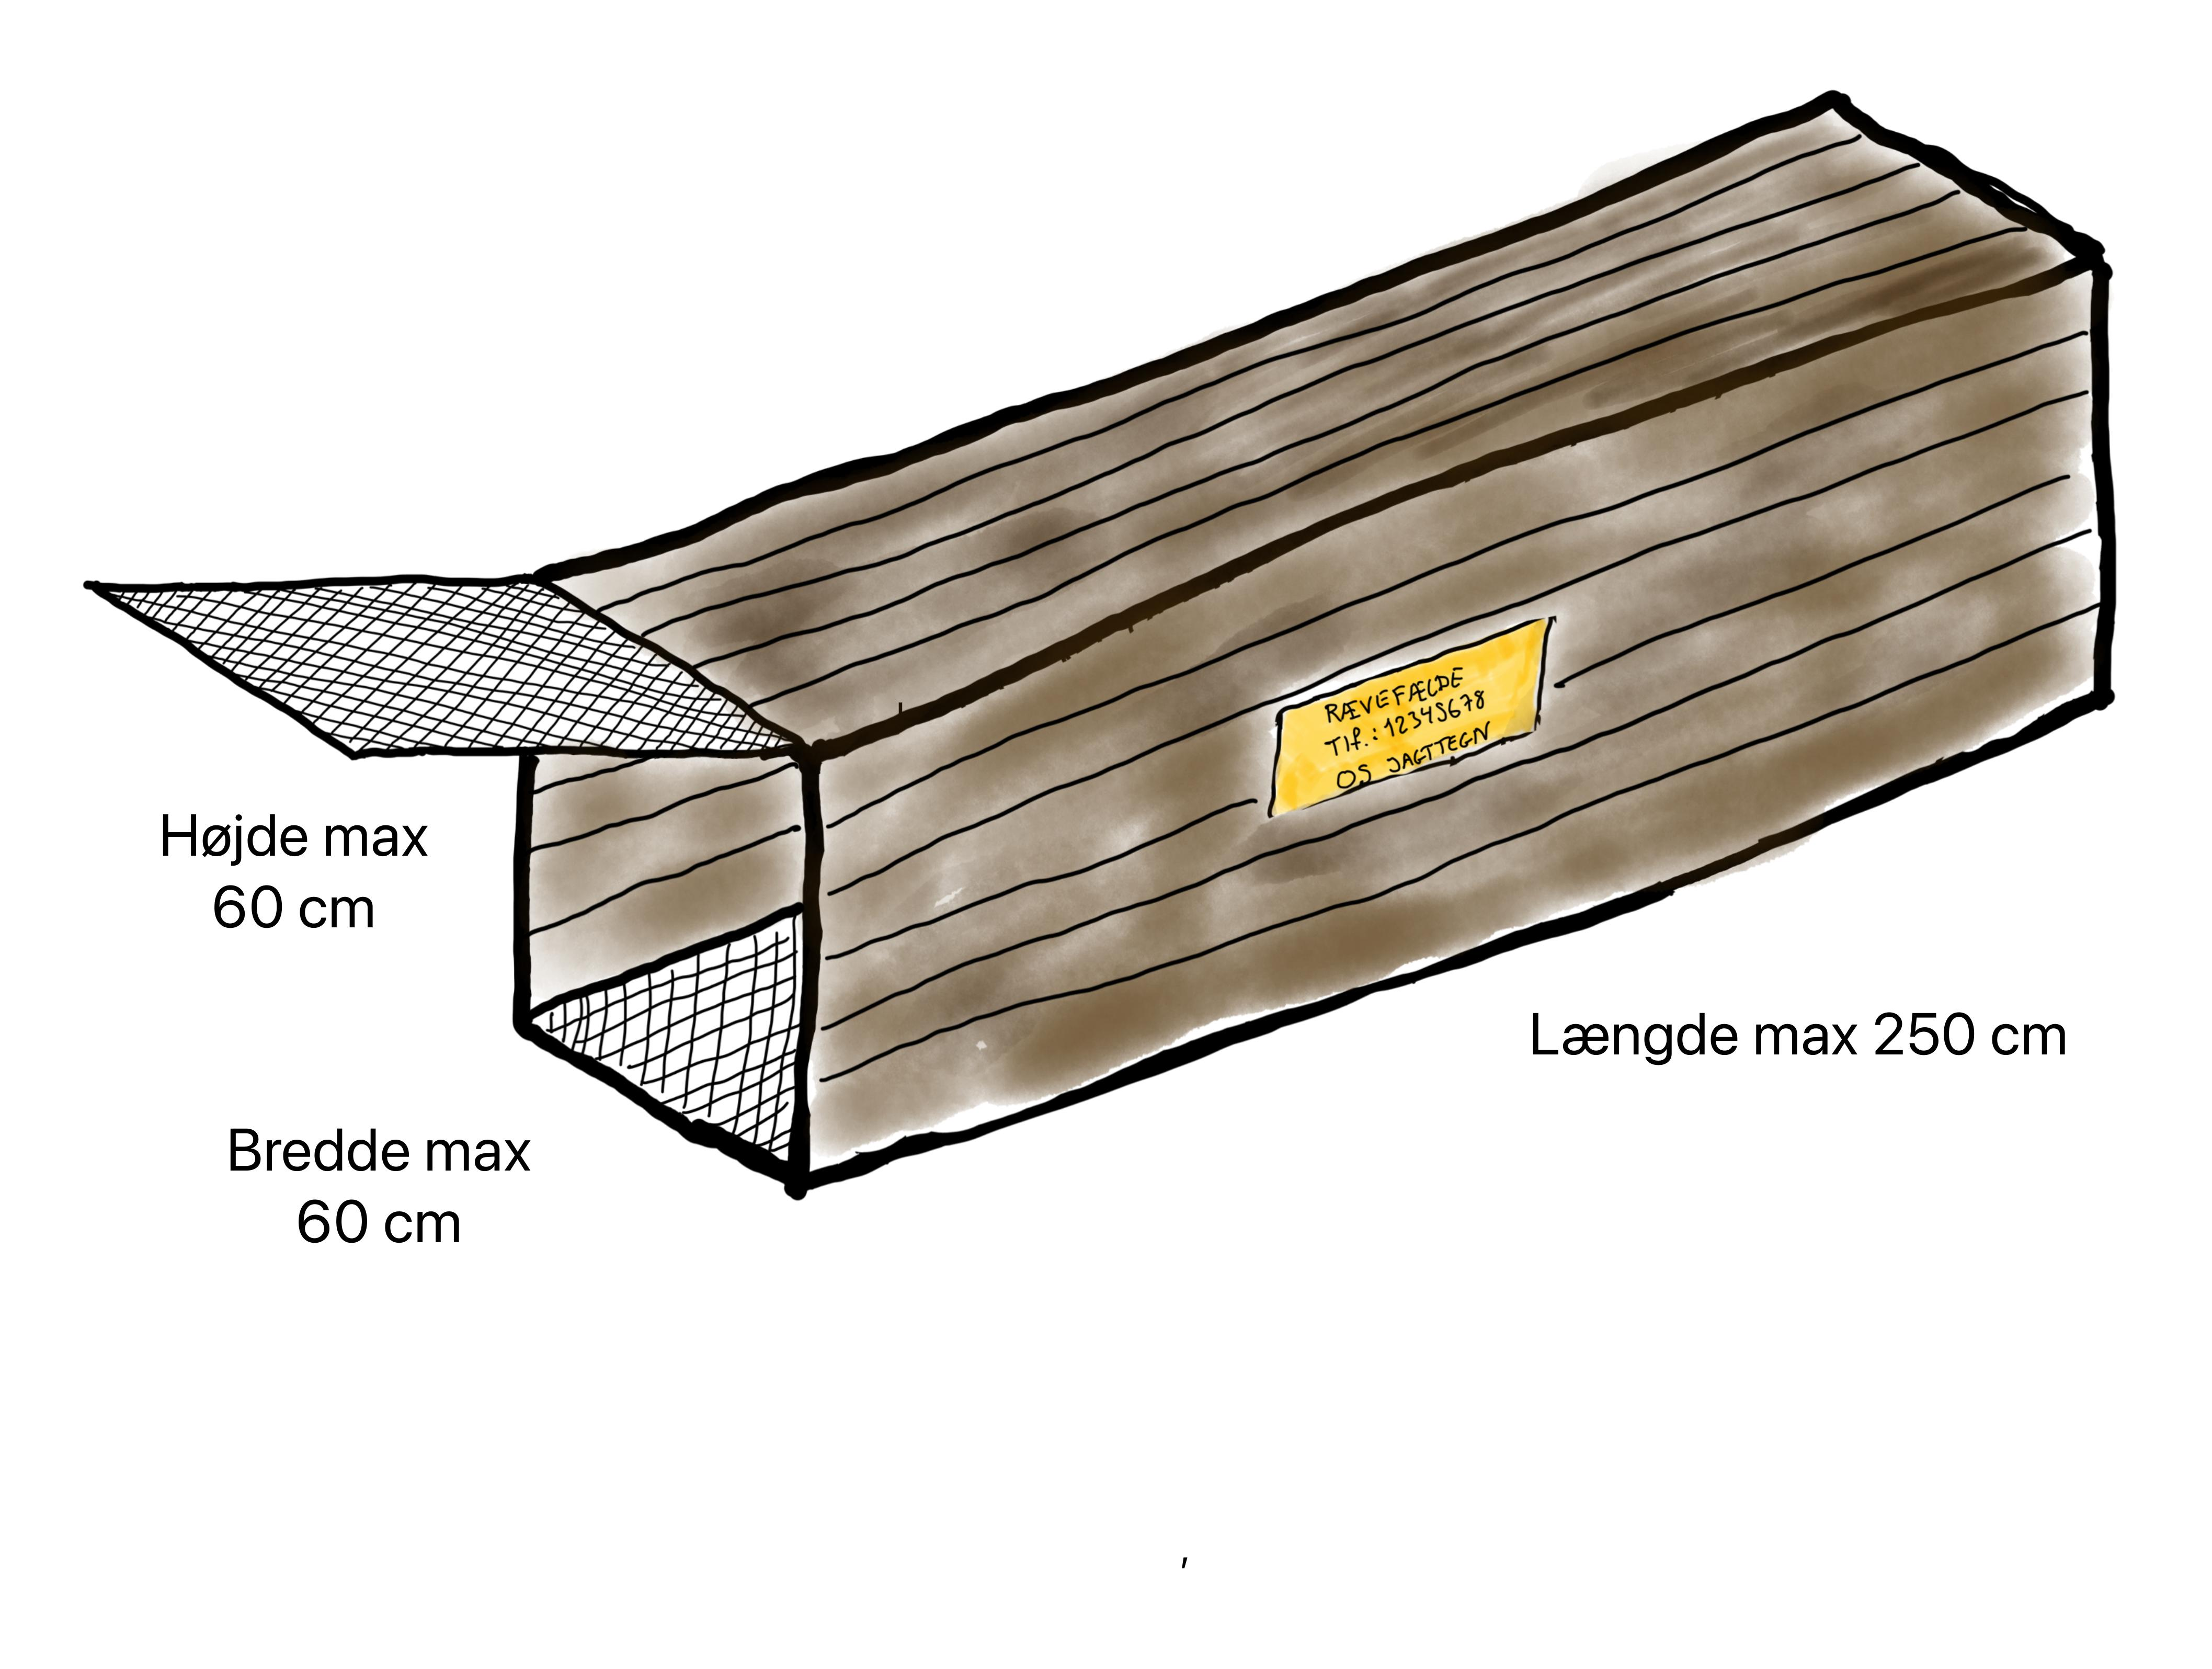
\includegraphics[width=\textwidth,height=0.75\textheight,keepaspectratio]{Billeder/Redskaber/raevefaelde.jpg}
% eller: [width=0.9\textwidth] hvis du vil have det lidt mindre

% Alternativt med figur-caption hvis du vil:
% \begin{figure}
%   \includegraphics[width=\textwidth]{dit_billede.jpg}
%   \caption{Eksempel på en rævefælde}
% \end{figure}

\end{column}

\end{columns}

\end{frame}

\begin{frame}{Brug af fælder til fugle (skrå sider)}

\begin{columns}[T]  % Top-aligned så tekst og billede starter i samme højde

\begin{column}{0.58\textwidth}  % Venstre: tekst (ca. 58 % bredde)
\vspace{1em}
\small
\raggedright

\begin{itemize}
\itemsep0.6em

\item Fangstrum max 60 (H) × 60 (B) × 250 (L) cm.

\item Indgangsåbninger ovenpå eller skråtstillet (40–50 grader). Ovenpå: Max 40 × 40 cm. Skrå: Max 60 × 40 cm.

\item Må ikke bruge kød eller ådsler som lokkemad.

\item Eftersyn morgen/aften kan erstattes af elektronisk enhed (f.eks. SMS-sender): Max 12 timer til fysisk tilsyn efter udløsning eller fejl. Fysisk tilsyn min. 1× dagligt første 3 dage.

\end{itemize}

\end{column}

\begin{column}{0.40\textwidth}  % Højre: billede (ca. 40 % bredde)
\centering
\vspace{0.5em}  % Lille top-margin for bedre balance

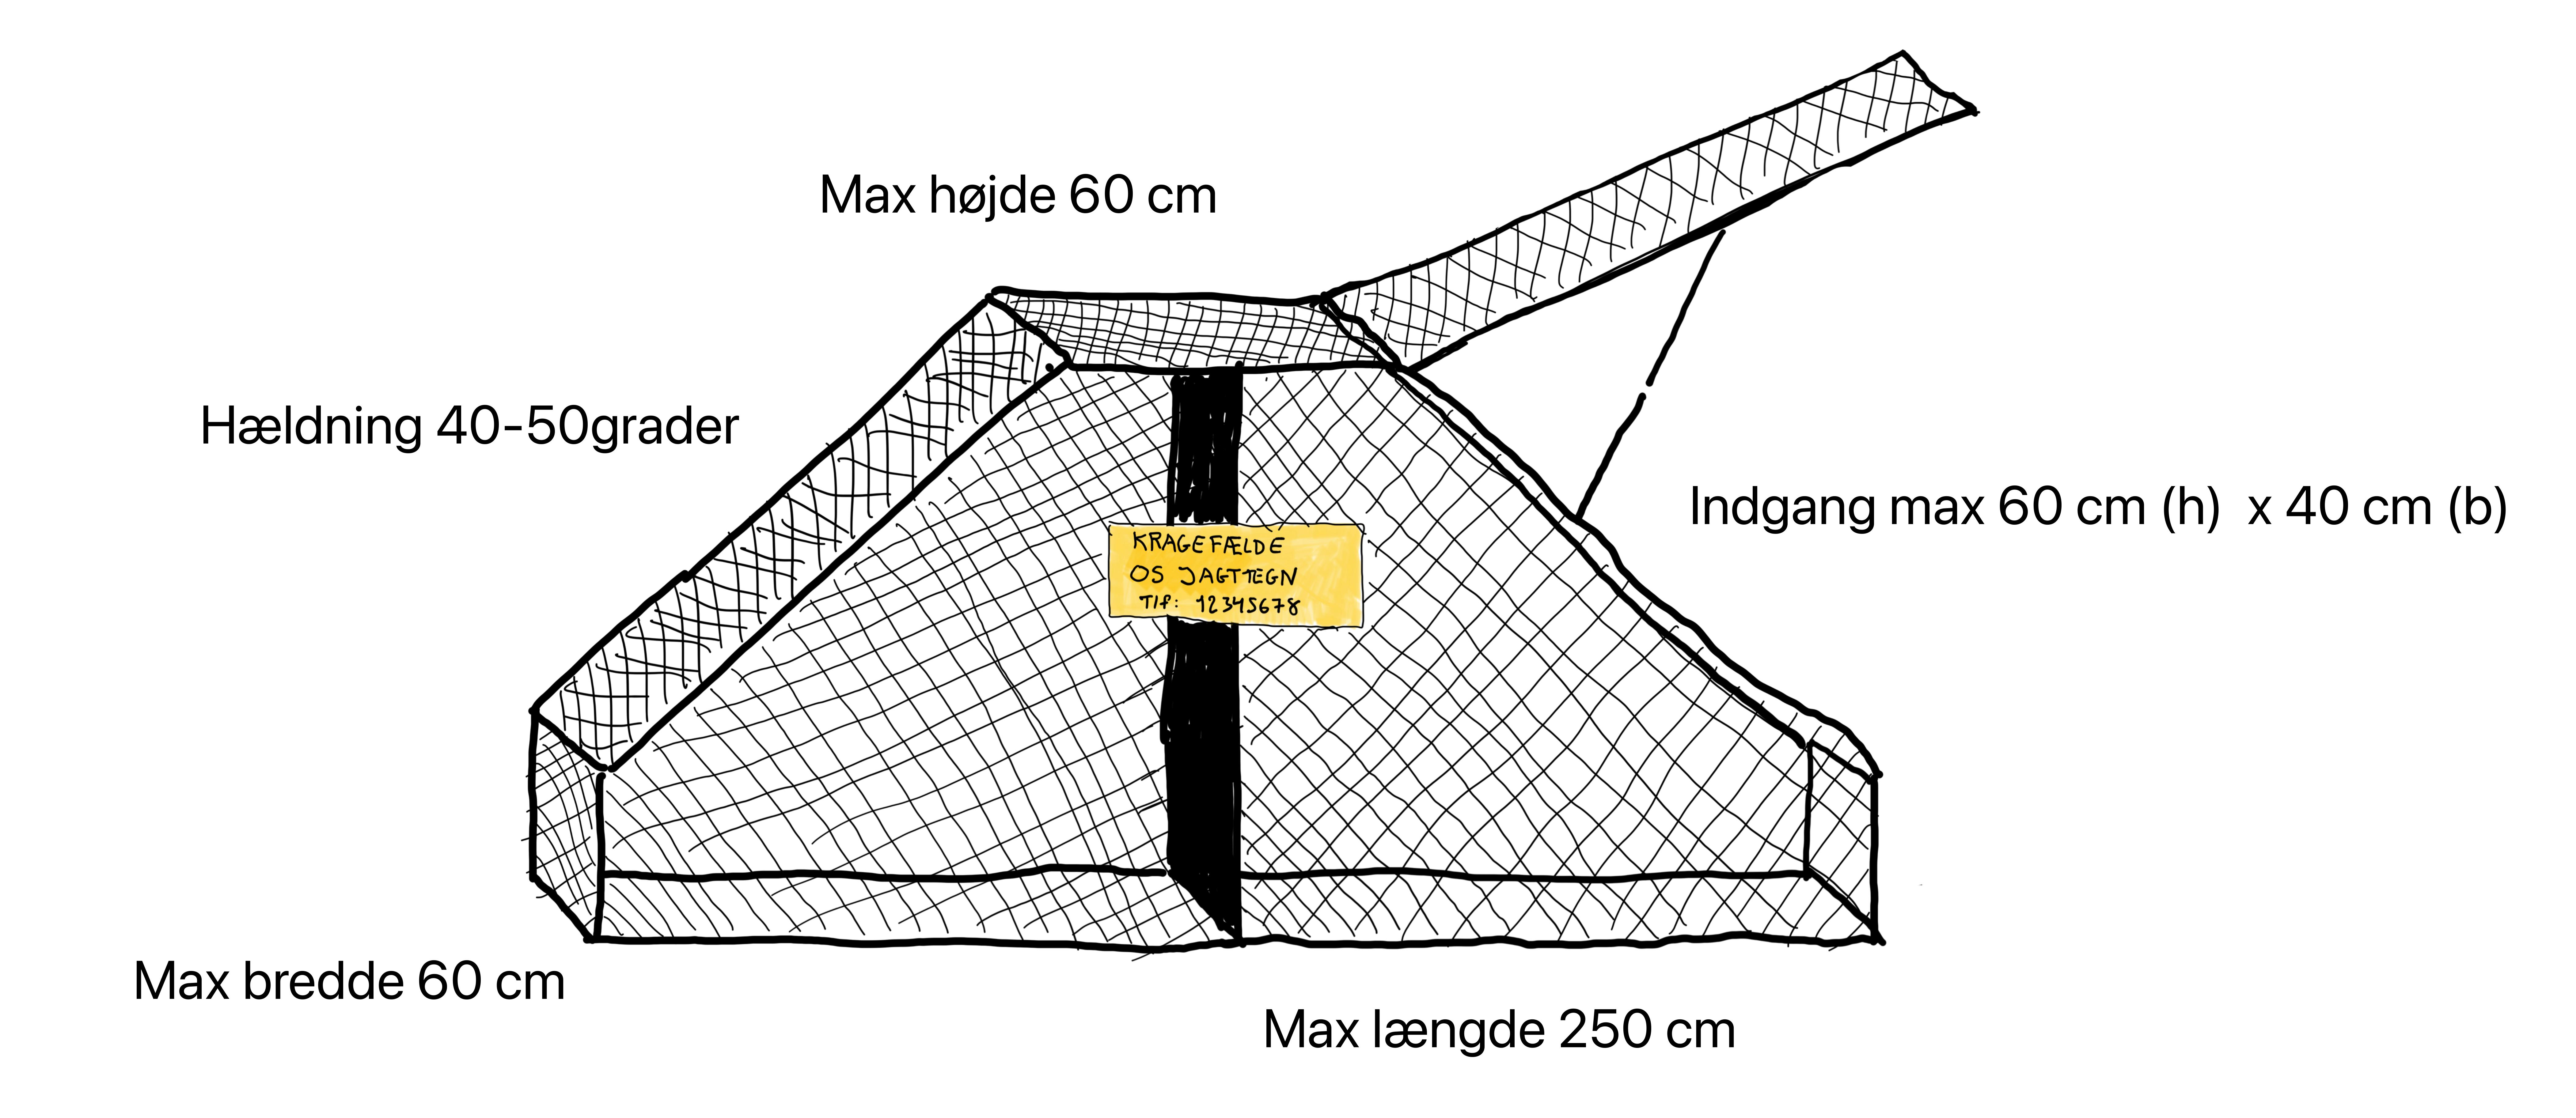
\includegraphics[width=\textwidth,height=0.75\textheight,keepaspectratio]{Billeder/Redskaber/fuglefaelde_skraa.jpg}
% Alternativer du kan prøve:
% \includegraphics[width=0.95\textwidth]{dit_billede.jpg}          % Lidt luft rundt om
% \includegraphics[height=0.7\textheight,keepaspectratio]{...}     % Begræns højde hvis billedet er højt

% Hvis du vil have en lille caption under billedet:
% \vspace{0.5em}
% \tiny Eksempel på fælde med skrå indgang (kilde: Naturstyrelsen eller lign.)

\end{column}

\end{columns}

\end{frame}

\begin{frame}{Brug af fælder til fugle (lige sider)}

\begin{center}
\vspace{0.5em}  % Lille top-margin for bedre balance på slide

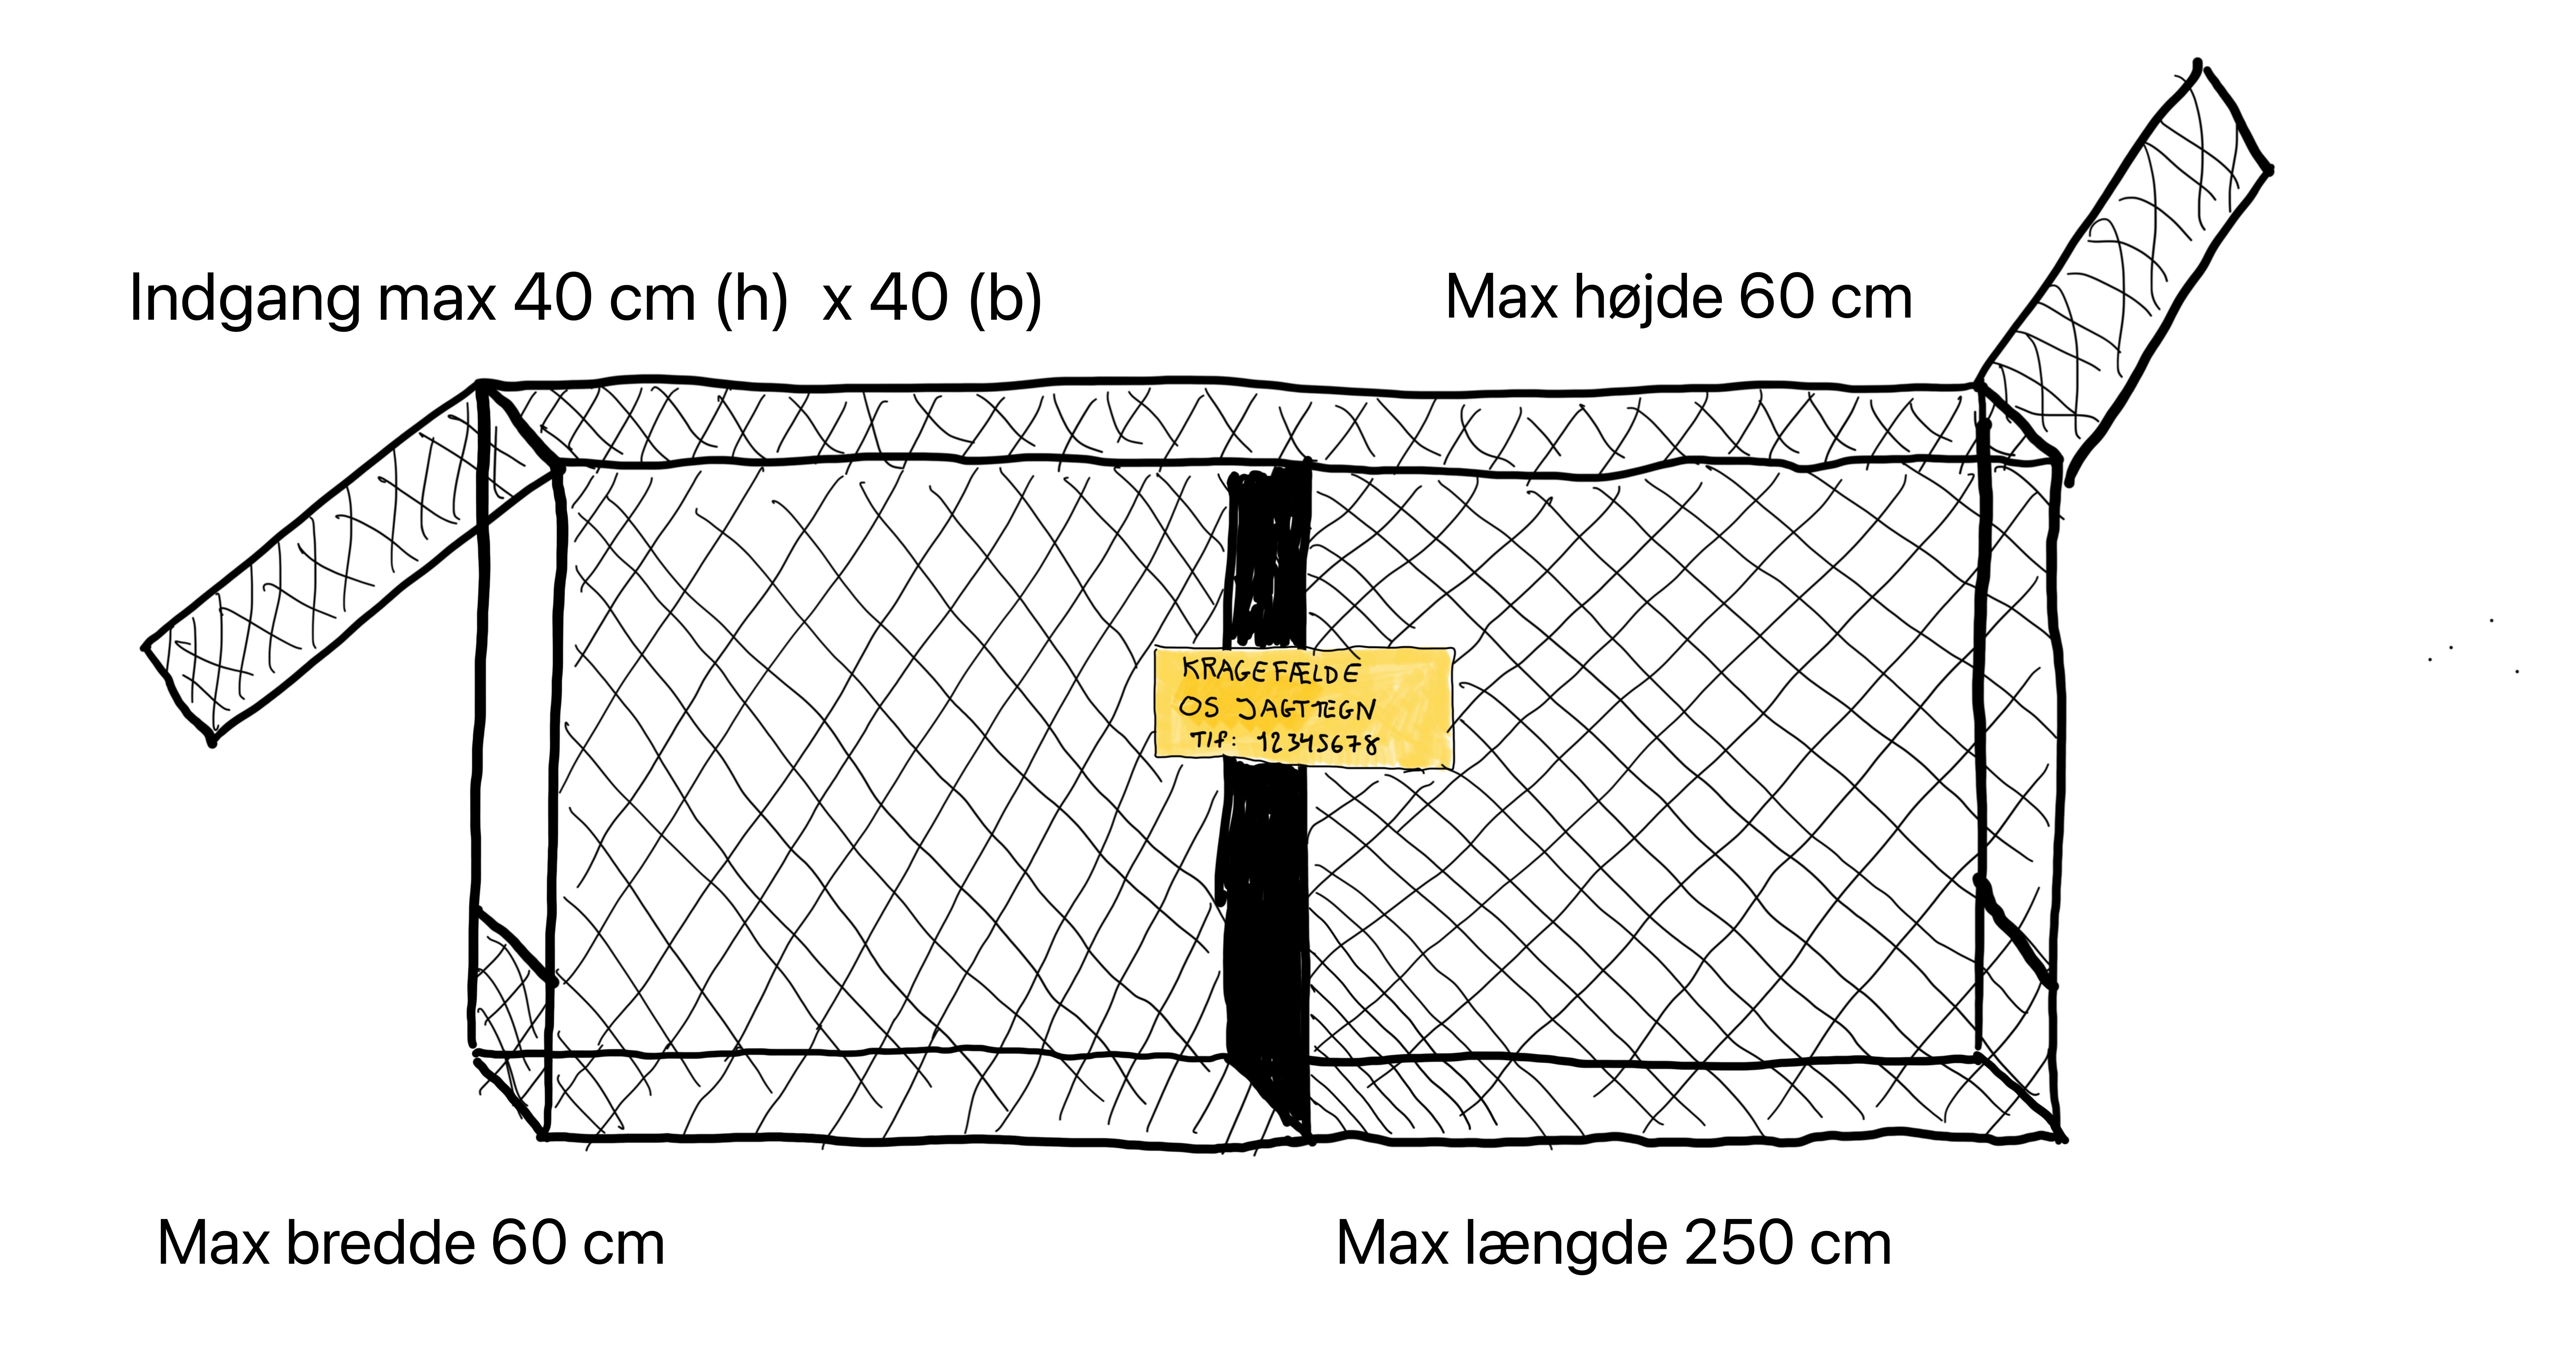
\includegraphics[height=0.85\textheight,keepaspectratio]{Billeder/Redskaber/fuglefaelde_lige.jpg}
% Alternativer du kan prøve for bedre pasform:
% \includegraphics[width=0.95\textwidth,keepaspectratio]{dit_billede.jpg}  % Bredde-prioriteret
% \includegraphics[width=\textwidth,height=0.8\textheight,keepaspectratio]{...}

% Valgfri lille caption under billedet (hvis du vil have det):
% \vspace{0.5em}
% \tiny Eksempel på fælde med skrå eller ovenpå-indgang (40–50 grader)

\end{center}

\end{frame}